\section{Experimental Results and Discussion}\label{sec:results}
To evaluate the performance of the GPU-accelerated C++/CUDA framework, we conduct comparative latency profiling, convergence analysis, and quantitative quality benchmarking between the classical Euclidean and quantum-inspired engines.

\subsection{Experimental Environment and Methodology}
All benchmarks are executed on a local system with an Intel Core Ultra 9 275HX CPU, 32~GB RAM, and an NVIDIA GeForce RTX 5070 Ti GPU (12~GB VRAM) under Windows 11. To ensure fair and reproducible comparisons, a global fixed-seed protocol (\texttt{STABLE\_RANDOM\_SEED = 42}) is implemented across the Mersenne Twister (\texttt{std::mt19937}) random initialization and the Monte Carlo silhouette sampling logic. Mathematical correctness is verified via a comprehensive GoogleTest suite targeting boundary conditions, empty cluster resilience, and CPU-GPU numerical parity (maintaining a $10^{-5}$ tolerance under floating-point drift).

\subsection{Latency Profiling and Throughput Scaling}
The system's execution latency is profiled across three standard operational modes under live camera processing: Performance ($K=3$, $S=8$), Balanced ($K=8$, $S=4$), and High Quality ($K=40$, $S=1$), where $K$ is the cluster count and $S$ is the downsampling stride. Table~\ref{tab:telemetry} details the stage-level latencies averaged over 21 runs.

\begin{table}[t]
\centering
\footnotesize
\caption{System Performance and Stage Latency Telemetry}
\label{tab:telemetry}
\begin{tabular}{ccccc}
\hline
\textbf{Mode} & \textbf{Preprocess} & \textbf{Optimize} & \textbf{Assign} & \textbf{Total Latency} \\ \hline
Performance  & 0.28 ms & 0.47 ms & 0.59 ms & \textbf{1.33 ms} \\
Balanced     & 0.29 ms & 0.74 ms & 0.59 ms & \textbf{1.62 ms} \\
High Quality & 0.30 ms & 2.93 ms & 0.62 ms & \textbf{3.86 ms} \\ \hline
\end{tabular}
\end{table}

The preprocessor kernel executes in $\approx 0.29\text{ ms}$ regardless of parameters due to 2D grid index efficiency. Centroid learning (optimization) scales with the active pixel count (stride $S$) and cluster count $K$, while pixel assignment scales minimally due to parallel thread occupancy. Across all modes, the pipeline achieves theoretical throughputs of $750\text{ FPS}$ (Performance), $618\text{ FPS}$ (Balanced), and $259\text{ FPS}$ (High Quality), vastly exceeding the real-time target of $120\text{ FPS}$ ($8.33\text{ ms}$ frame budget) and leaving substantial processing headroom under live 30 FPS video feeds.

Table~\ref{tab:latency_benchmarks} evaluates average execution latency and convergence iteration counts under a highly textured static workspace over 21 trials (using K-Means++ seeding) to evaluate GPU scaling under heavy workloads.

\begin{table}[b]
\centering
\small
\caption{Performance Comparison of Classical vs. Quantum K-Means}
\label{tab:latency_benchmarks}
\begin{tabular}{ccccc}
\hline
\textbf{Mode} & \multicolumn{2}{c}{\textbf{Classical}} & \multicolumn{2}{c}{\textbf{Quantum}} \\
 & \textbf{Lat. (ms)} & \textbf{Iter.} & \textbf{Lat. (ms)} & \textbf{Iter.} \\ \hline
Performance  & 1.8056  & 11.71  & 1.6107  & 12.38  \\
Balanced     & 6.4545  & 41.81  & 6.1547  & 41.43  \\
High Quality & 26.6608 & 88.67  & 27.9470 & 88.62  \\ \hline
\end{tabular}
\end{table}

Under low-density and balanced loads, the quantum-inspired engine is slightly faster ($1.61\text{ ms}$ vs. $1.81\text{ ms}$ and $6.15\text{ ms}$ vs. $6.45\text{ ms}$). This is driven by SFU hardware-accelerated cosine intrinsics. Under high density ($K=40, S=1$), the classical engine is slightly faster ($26.66\text{ ms}$ vs. $27.95\text{ ms}$). Despite trigonometric calculations, the engines maintain near-parity due to global VRAM fetch latencies dominating overall execution, allowing the GPU to hide arithmetic overhead by scheduling warps.

\subsection{Quantitative Clustering Quality and Lighting Telemetry}
Clustering quality was evaluated on a static VGA frame under two illumination environments: Scene A (uniform studio lighting) and Scene B (dim room with monitor glow and high sensor noise). Table~\ref{tab:quality_metrics} details the quality diagnostics under the balanced configuration ($K=8$, $S=4$, 21-run average).

\begin{table}[t]
\centering
\footnotesize
\caption{Segmentation Quality and Telemetry under Varying Lighting}
\label{tab:quality_metrics}
\setlength{\tabcolsep}{4pt}
\begin{tabular}{lccccc}
\hline
\textbf{Engine} & \textbf{Lat. (ms)} & \textbf{Iter.} & \textbf{WCSS} & \textbf{$\mathcal{D}\mathcal{B}$} & \textbf{Sil.} \\ \hline
\multicolumn{6}{l}{\textbf{Scene A (Studio)}} \\
\quad Classical & 5.4841 & 36.48 & 2189.43 & 0.68200 & 0.48335 \\
\quad Quantum   & 5.3617 & 35.81 & 2189.49 & 0.68194 & 0.48338 \\ \hline
\multicolumn{6}{l}{\textbf{Scene B (Low-Light)}} \\
\quad Classical & 2.7696 & 18.38 & 711.41  & 0.65632 & 0.54520 \\
\quad Quantum   & 2.9941 & 18.33 & 711.42  & 0.65636 & 0.54527 \\ \hline
\end{tabular}
\end{table}

The quantum-inspired engine achieves mathematical parity with the classical Euclidean solver: WCSS differs by less than $0.003\%$, while the Davies-Bouldin index and Silhouette scores align within $10^{-4}$. This is because the cosine-squared mapping remains monotonic within $[0, \pi/4]$, preserving the relative ordering of feature distances and converging to the same local minima. Thus, the non-linear Hilbert phase space mapping is a mathematically robust alternative that does not degrade class discrimination under noisy conditions.

\subsection{Visual Quality and Temporal Stability}
Full-frame segmentations (shown in Fig.~\ref{fig:case_study_1}) verify that both backends produce visually identical segment boundaries under both studio and low-light conditions.

\begin{figure}[b]
\centering
\begin{minipage}{0.32\columnwidth}
  \centering
  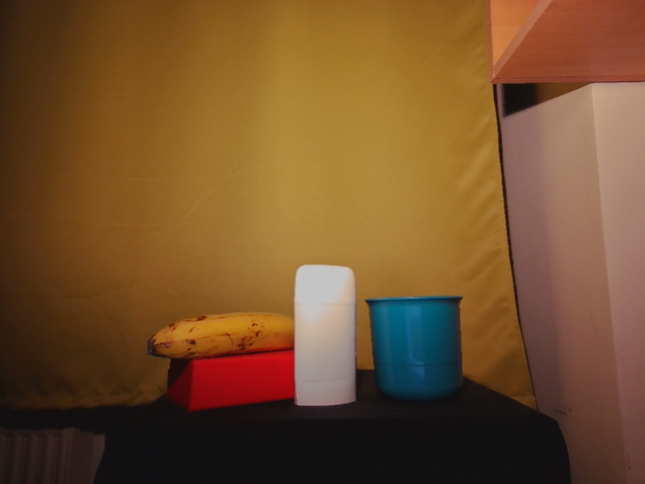
\includegraphics[width=\textwidth]{figures/scene_a.png}
  \vspace{0.1em}
  {\scriptsize Original (A)}
\end{minipage}\hfill
\begin{minipage}{0.32\columnwidth}
  \centering
  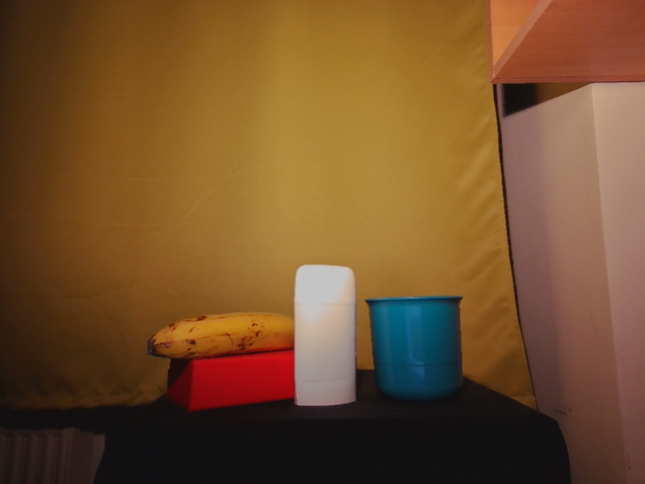
\includegraphics[width=\textwidth]{figures/scene_a.png}
  \vspace{0.1em}
  {\scriptsize Classical (A)}
\end{minipage}\hfill
\begin{minipage}{0.32\columnwidth}
  \centering
  
\includegraphics[width=\textwidth]{figures/scene_a_quantum.png}
  \vspace{0.1em}
  {\scriptsize Quantum (A)}
\end{minipage}

\vspace{0.3em}

\begin{minipage}{0.32\columnwidth}
  \centering
  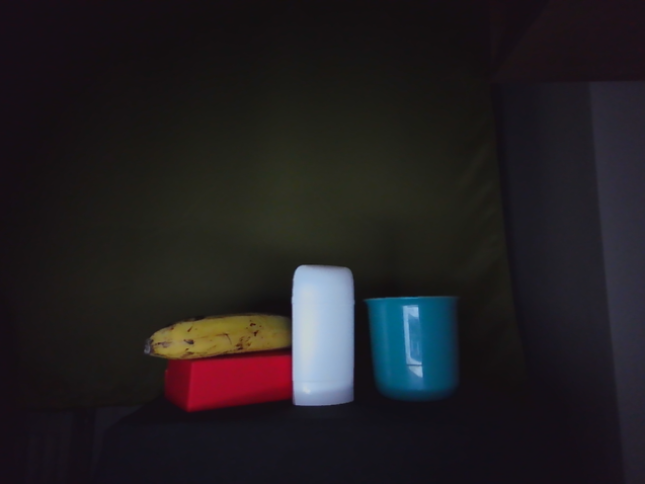
\includegraphics[width=\textwidth]{figures/scene_b.png}
  \vspace{0.1em}
  {\scriptsize Original (B)}
\end{minipage}\hfill
\begin{minipage}{0.32\columnwidth}
  \centering
  
\includegraphics[width=\textwidth]{figures/scene_b_classical.png}
  \vspace{0.1em}
  {\scriptsize Classical (B)}
\end{minipage}\hfill
\begin{minipage}{0.32\columnwidth}
  \centering
  
\includegraphics[width=\textwidth]{figures/scene_b_quantum.png}
  \vspace{0.1em}
  {\scriptsize Quantum (B)}
\end{minipage}
\caption{Visual Segmentations for Scenes A and B ($K=8$, $S=4$)}
\label{fig:case_study_1}
\end{figure}

The spatial weight parameter ($\lambda_{\text{spatial}} = 10^{-6}$) acts as a regularizer. Setting it too low allows color sensor noise to dominate and fragment clusters, whereas setting it too high forces grid-like partitions that ignore contours. The balanced spatial weighting prevents boundary noise while preserving sharp edge details in both backends. 

Under live video loops, frame-by-frame independent clustering results in temporal jitter. Jitter sequences reveal that random variations in initialization seeding cause both engines to allocate clusters differently between consecutive frames (e.g., shifting cluster assignments on flat background regions, which reduces the centroids available for resolving fine foreground detail). This identical shift confirms that temporal consistency is dominated by initial seeding strategies rather than the underlying metric topography.
